\documentclass[11pt,a4paper]{article}

\usepackage[margin=1in]{geometry}
\usepackage{graphicx}
\usepackage[hidelinks]{hyperref}
\usepackage{booktabs}
\usepackage{listings}
\usepackage{xcolor}
\usepackage{caption}
\usepackage{float}
\usepackage{amsmath}
\usepackage{microtype}
\usepackage{enumitem}
\usepackage[british]{babel}
\usepackage{parskip}

% ---------- code listing style ----------
\definecolor{codegray}{rgb}{0.96,0.96,0.96}
\definecolor{codeblue}{rgb}{0.13,0.29,0.53}
\definecolor{codegreen}{rgb}{0.00,0.50,0.00}
\definecolor{codecomment}{rgb}{0.50,0.50,0.50}

\lstset{
  basicstyle=\ttfamily\footnotesize,
  backgroundcolor=\color{codegray},
  keywordstyle=\color{codeblue}\bfseries,
  stringstyle=\color{codegreen},
  commentstyle=\color{codecomment}\itshape,
  breaklines=true,
  showstringspaces=false,
  frame=single,
  rulecolor=\color{gray!30},
  language=Python,
  xleftmargin=1em,
  xrightmargin=1em,
}

\title{\vspace{-2em}\textbf{Predicting Gene Expression Levels from Human Coding Sequences with a Custom Transformer}}
\author{Arnab Satyam Roy \\
MSc Bioinformatics, American International University -- Bangladesh}
\date{May 2026}

\begin{document}
\maketitle
\vspace{-1em}

% ====================================================================
\section*{Executive Summary}

How strongly a gene is expressed in a given tissue is one of the most basic quantities in molecular biology, and one of the hardest to predict from sequence alone. The bulk of the regulatory signal sits outside the gene itself: in promoter regions, enhancers, untranslated regions, and chromatin context. This project asks a deliberately narrow version of the prediction problem. Given only a gene's protein-coding sequence, with no access to any of those regulatory regions, how well can a Transformer-based classifier sort that gene into one of three expression bins (Low, Medium, High) calibrated against liver tissue?

The pipeline links 12{,}051 human protein-coding genes from NCBI with median TPM values from GTEx v8, derives three balanced expression classes by percentile binning, and feeds 6-mer-tokenised sequences into a custom encoder-only Transformer. On a held-out test set of 2{,}411 genes the model reaches an accuracy of 0.634, a macro-F1 of 0.634, and a one-vs-rest AUROC of 0.806. Two interpretability tools, attention rollout and input-gradient saliency, surface the k-mers each prediction relied on, and a FastAPI service exposes the whole system through a small HTML/CSS/JS frontend.

The headline accuracy is honest-middling. We treat that as a methodologically meaningful finding rather than a weakness: the model is performing roughly where one would expect it to perform when the input deliberately excludes the regulatory regions that biology says do the heavy lifting.

% ====================================================================
\section{Introduction and Motivation}

\subsection{Background}

Gene expression governs which proteins a cell produces and, consequently, what that cell does. Two cells with identical DNA can behave entirely differently because their expression profiles diverge. A hepatocyte and a neuron share the same genome but inhabit very different molecular worlds. Sequencing technologies such as RNA-seq let researchers measure expression directly, and consortia like GTEx have published tissue-resolved expression atlases covering tens of thousands of genes. Predicting expression from sequence alone, without doing the experiment, has proved much harder.

Most of what we know about transcriptional regulation lives outside the gene body. Promoter sequences a few hundred base pairs upstream of a transcription start site contain binding motifs for transcription factors. Distal enhancers can sit hundreds of kilobases away and still loop in to drive expression. Chromatin state, methylation patterns, and three-dimensional genome architecture all matter. Coding sequences, the parts that actually become protein, are not the obvious place to look for the strongest expression-predictive signal.

That makes the problem interesting rather than hopeless. If a model can extract any expression-predictive signal from coding sequence alone, that signal will plausibly come from codon usage bias, GC content, sequence composition tied to translational efficiency, or the occasional regulatory element embedded in a coding region. Measuring how far a model can be pushed using only this restricted input is useful on its own terms. It quantifies how much of the prediction problem the coding sequence is actually carrying.

\subsection{Problem Statement}

Given a human protein-coding gene's nucleotide sequence, and nothing else, can a Transformer-based classifier reliably place that gene into one of three expression-level classes (Low, Medium, or High) in liver tissue?

\subsection{Objectives}

\begin{enumerate}[itemsep=2pt]
    \item Assemble a labelled dataset linking NCBI human coding sequences to GTEx median TPM values, with identifier harmonisation through Ensembl and HGNC symbols.
    \item Convert continuous expression values into three balanced ordinal classes by percentile binning, so the task is well-posed and the chance baseline is unambiguous.
    \item Train a custom encoder-only Transformer over 6-mer-tokenised sequences and report classification metrics on a held-out test set.
    \item Add interpretability tools (attention rollout and input-gradient saliency) so individual predictions can be inspected at the level of single 6-mers.
    \item Deploy the trained model behind a small FastAPI service with a static frontend, suitable for live demonstration and inspection.
\end{enumerate}

% ====================================================================
\section{Dataset Description}

\subsection{Data Source}

Three public resources back the dataset. Human protein-coding sequences come from the National Center for Biotechnology Information's (NCBI) gene database, queried programmatically and filtered to ACGT-only records of length up to 1{,}000 base pairs. Expression labels come from the Genotype-Tissue Expression (GTEx) v8 release, specifically the per-tissue median TPM table. The default tissue for training and evaluation is liver, chosen for its high coverage in the GTEx atlas and its biologically distinct expression profile. Cross-resource identifier harmonisation, mapping between NCBI Entrez gene IDs, Ensembl gene IDs, and HGNC symbols, is handled through the MyGene.info REST API.

\subsection{Data Cleaning and Preprocessing}

The raw download yields a large pool of sequences, many of them noisy. Alternate splice variants, records containing IUPAC ambiguity codes (N, R, Y, and similar), and extremely long entries are common. We applied three filters in order. First, sequences with any character outside \{A, C, G, T\} were dropped. Second, sequences longer than 1{,}000 base pairs were excluded so that positional encoding range and attention cost stayed manageable on consumer hardware; this trims the dataset further and biases it toward shorter genes, often single-exon transcripts. Third, sequences without a successful join to a GTEx TPM value were dropped after the identifier mapping step.

Raw TPM values are heavily right-skewed. A small number of housekeeping and tissue-specific genes (haemoglobin in blood, albumin in liver, and so on) inflate the upper tail. We applied a $\log(\text{TPM} + 1)$ transform and then computed the 33rd and 67th percentiles across the full dataset, with rank-based assignment to handle the many genes tied at TPM = 0. Genes below the 33rd percentile became \texttt{Low}, those between the two thresholds became \texttt{Medium}, and those above the 67th percentile became \texttt{High}. Binning on percentiles produces three approximately equal-sized classes by construction, which makes downstream analysis cleaner: the chance baseline is a flat 33.3\%, and accuracy and macro-F1 can be read directly without class re-weighting at evaluation time.

After all filtering and joining, 12{,}051 genes remained. We held out 2{,}411 of these (20\% of the cleaned dataset) as a stratified test set, and split the remaining records into training and validation portions, again stratified by class.

\begin{figure}[H]
\centering
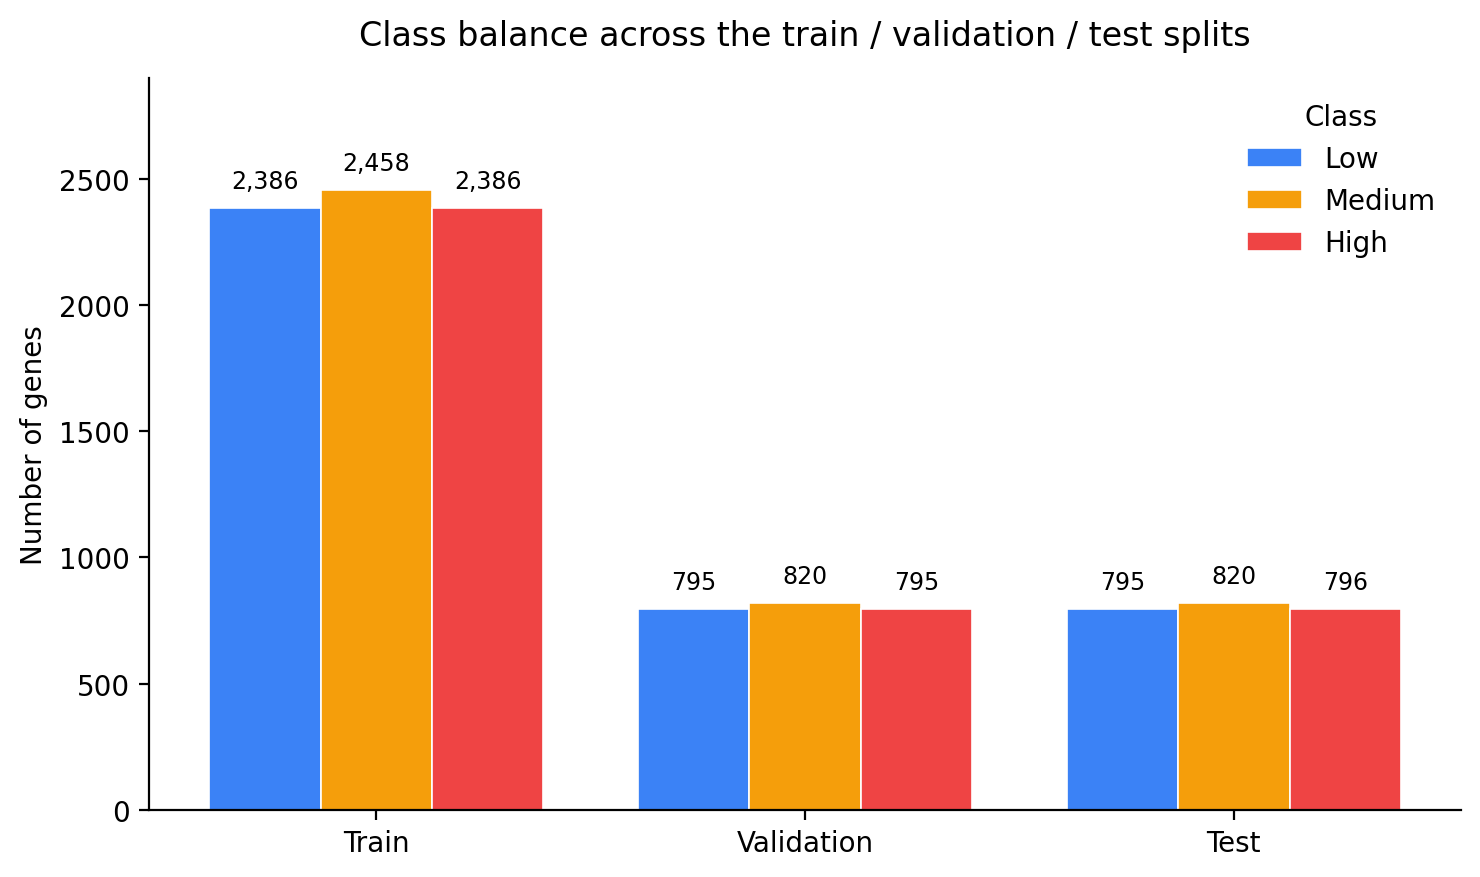
\includegraphics[width=0.85\textwidth]{figures/class_distribution.png}
\caption{Class balance across the three splits. Percentile-based binning produces near-identical class sizes within each split, so accuracy and macro-F1 can be read against a 33.3\% chance baseline without re-weighting.}
\label{fig:class_dist}
\end{figure}

\subsection{Variables}

\begin{table}[H]
\centering
\begin{tabular}{@{}lll@{}}
\toprule
\textbf{Variable} & \textbf{Type} & \textbf{Description} \\
\midrule
\texttt{gene\_id} & Categorical & NCBI Entrez gene identifier. \\
\texttt{gene\_symbol} & Categorical & Official HGNC symbol (for example \emph{HBA1}, \emph{IFNB1}). \\
\texttt{sequence} & String & Protein-coding nucleotide sequence over $\{$A, C, G, T$\}$. \\
\texttt{median\_tpm} & Quantitative & GTEx v8 median TPM in liver tissue. \\
\texttt{log\_tpm} & Quantitative & $\log(\text{median\_tpm} + 1)$. \\
\texttt{expression\_label} & Ordinal & Class derived from \texttt{log\_tpm}: Low, Medium, or High. \\
\bottomrule
\end{tabular}
\caption{Schema of the final labelled dataset.}
\label{tab:schema}
\end{table}

% ====================================================================
\section{Methodology and Tools}

\subsection{Tools Used}

The stack is deliberately small. PyTorch handles model construction and training; the encoder itself is built directly on \texttt{torch.nn.TransformerEncoderLayer} rather than imported as a higher-level abstraction. Pandas and NumPy do the data wrangling, Biopython parses FASTA records, and the \texttt{mygene} Python client wraps the MyGene.info API for identifier mapping. Scikit-learn provides the classification metrics (precision, recall, F1, ROC AUC, confusion matrix). Matplotlib and seaborn produce the figures, and FastAPI with Uvicorn serves the trained model behind a static HTML/CSS/JS frontend.

\subsection{Tokenisation}

DNA cannot be fed straight into a Transformer; it has to be discretised. We chose a 6-mer tokeniser, sliding a window of width six along each sequence with a stride of one and emitting the corresponding substring at each step. A sequence of length $L$ therefore produces $L - 5$ tokens. The vocabulary contains $4^6 = 4{,}096$ possible 6-mers plus three special tokens (\texttt{[PAD]} for padding, \texttt{[UNK]} for unknown k-mers, and \texttt{[CLS]} for the sequence-level representation), giving 4{,}099 entries in total. The choice of $k = 6$ is conventional for DNA modelling work. It captures enough local context to encode short regulatory and codon-level motifs while keeping the vocabulary tractable.

\subsection{Model Architecture}

The classifier is a pre-LayerNorm encoder-only Transformer. Tokens are projected to a 128-dimensional embedding space, summed with sinusoidal positional encodings, and passed through four \texttt{TransformerEncoderLayer} blocks. Each block has four attention heads, a feed-forward dimension of 256, and a dropout rate of 0.1. A \texttt{[CLS]} token prepended to every input acts as the aggregator; its final-layer hidden state is layer-normalised, dropped out at 0.1, and projected through a single linear layer to three class logits. Total parameter count is approximately 1.1 million. The model is small on purpose: training a much larger network on a dataset of 12{,}052 sequences risks overfitting more than it adds capacity in the useful direction.

\begin{figure}[H]
\centering
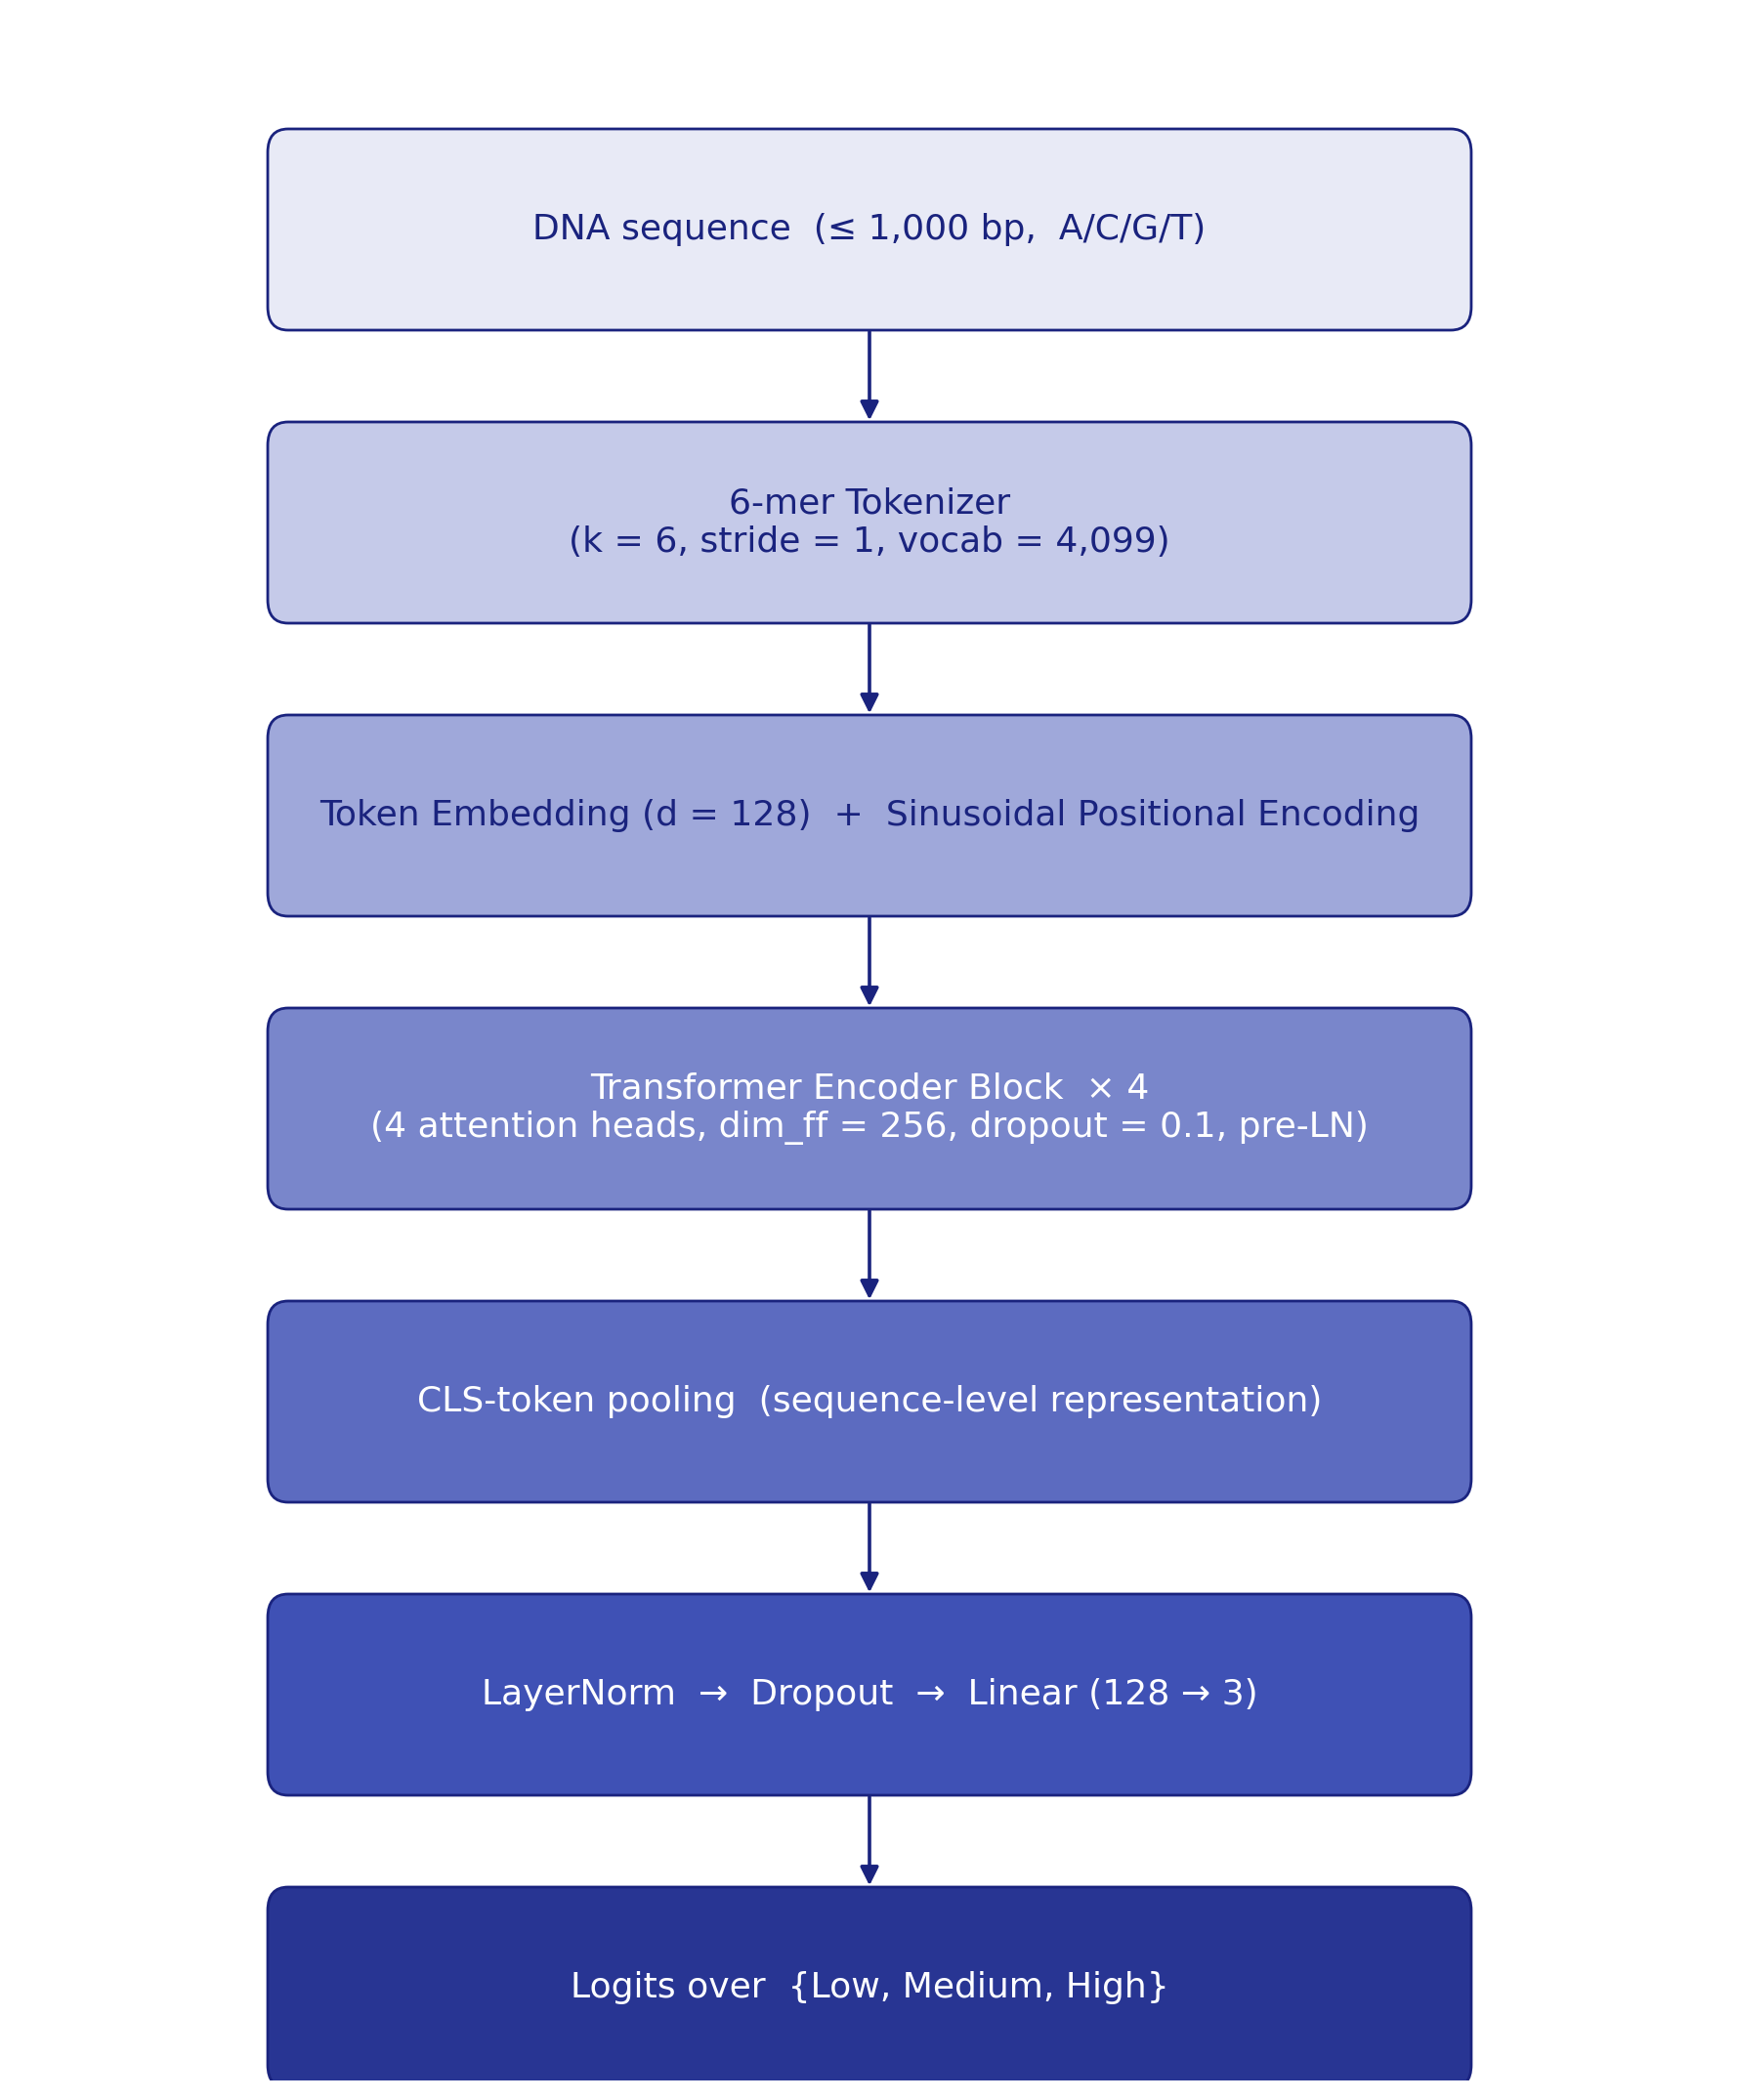
\includegraphics[width=0.70\textwidth]{figures/architecture_diagram.png}
\caption{Model architecture. The input DNA sequence is tokenised into overlapping 6-mers, embedded with sinusoidal position encodings, passed through four pre-LayerNorm Transformer blocks, and read out from a learned \texttt{[CLS]} token.}
\label{fig:arch}
\end{figure}

\subsection{Training Setup}

Loss is class-weighted cross-entropy with label smoothing $\alpha = 0.1$. The class weights are not strictly necessary given the balanced binning, but they are retained as a safety margin against any minor imbalance introduced by the stratified split. Reverse-complement augmentation is applied with probability 0.5: at each training step, with even odds, the input sequence is replaced by its reverse complement before tokenisation. This encodes a useful prior, since a coding sequence and its reverse complement are biologically related, and it roughly doubles the effective size of the training set.

The optimiser is AdamW with learning rate $1 \times 10^{-3}$ and weight decay $1 \times 10^{-4}$. A three-epoch linear warmup is followed by cosine annealing across the remaining 27 epochs. Gradient norms are clipped at 1.0 to keep early updates from destabilising training. Batch size is 16, set primarily by GPU memory rather than by tuning. We trained for 30 epochs and retained the checkpoint with the best validation accuracy.

\subsection{Interpretability}

Two complementary tools accompany the classifier.

\textbf{Attention rollout} (Abnar and Zuidema, 2020) propagates self-attention through layers. At each block the raw attention matrix is corrected for the residual connection and the corrected matrices are multiplied together across layers, yielding an estimate of how much information flows from every input token up to the \texttt{[CLS]} aggregator at the top of the stack. The result is a vector of importance scores, one per 6-mer, that can be rendered as a heatmap over the original sequence.

\textbf{Input-gradient saliency} computes the gradient of the predicted class logit with respect to the input token embeddings, then takes an element-wise product with the embeddings themselves. The ``input times gradient'' formulation produces a complementary importance score per 6-mer that is sensitive to features the attention rollout can miss, particularly features carried through the feed-forward sublayers rather than the attention mechanism.

We report both because neither alone is a reliable explanation. Attention is not necessarily explanation, and gradient methods are well known to be noisy. Showing two views, and pointing out where they agree or disagree, is more honest than picking one and treating it as ground truth.

\subsection{Web Application}

FastAPI exposes three endpoints. \texttt{GET /} returns the static frontend. \texttt{POST /predict} takes a JSON body of the form \texttt{\{"sequence": "ACGT..."\}}, runs inference, and returns the predicted class, the full class-probability vector, the attention-rollout scores, and the saliency scores. \texttt{GET /health} returns a small status payload used for sanity checks. The frontend is plain HTML, CSS, and vanilla JavaScript with no build step or framework, which keeps the deployment friction low and makes the project easy to demonstrate offline.

% ====================================================================
\section{Visualisations and Key Findings}

\subsection{Training Dynamics}

Training loss falls steadily; validation loss flattens out before the run ends. Macro-F1 on the validation set climbs into the low 0.6s and stays there. We did not see runaway overfitting, which is plausibly an effect of label smoothing, dropout, and reverse-complement augmentation working together. The model also does not break through its plateau. We argue in the limitations section that this is the information ceiling rather than a tuning failure.

\subsection{Test Set Performance}

\begin{table}[H]
\centering
\begin{tabular}{@{}lc@{}}
\toprule
\textbf{Metric} & \textbf{Value} \\
\midrule
Test accuracy & 0.634 \\
Macro-F1 & 0.634 \\
AUROC (one-vs-rest, macro-averaged) & 0.806 \\
Test set size & 2{,}411 \\
\bottomrule
\end{tabular}
\caption{Headline test-set metrics for the trained Transformer.}
\label{tab:results}
\end{table}

\begin{figure}[H]
\centering
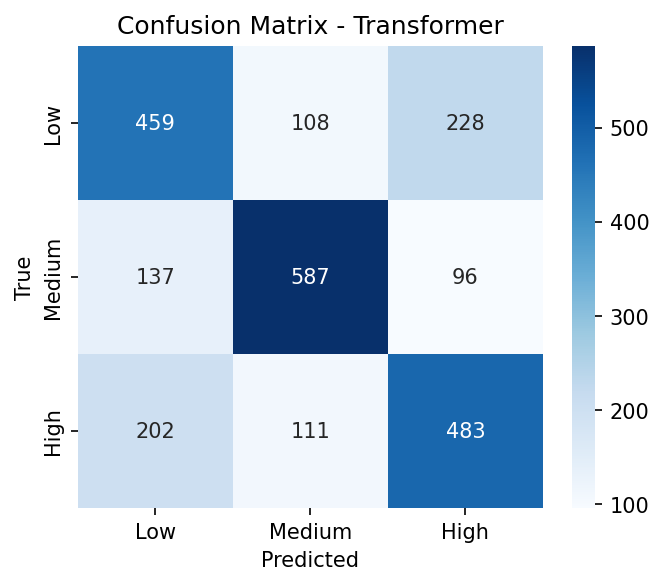
\includegraphics[width=0.55\textwidth]{figures/confusion_matrix.png}
\caption{Confusion matrix on the test set ($n = 2{,}411$). Most confusion is between adjacent classes (Low/Medium and Medium/High); confusion across the two extreme classes is rare.}
\label{fig:confusion}
\end{figure}

\textbf{Interpretation.} An accuracy of 0.634 on a three-class balanced problem is nearly twice the chance baseline of 0.333. The structure of the confusion matrix is more informative than the headline number. Off-diagonal mass concentrates next to the true class: Low is most often confused with Medium and Medium with High, while errors that jump across two classes (Low predicted as High, or vice versa) are uncommon. The model has clearly picked up an ordinal signal in the expression distribution, even though the cross-entropy loss treats the classes as nominal. That is the pattern one would expect from a model that knows roughly where on the expression scale a gene sits but cannot pin the answer down precisely.

\begin{figure}[H]
\centering
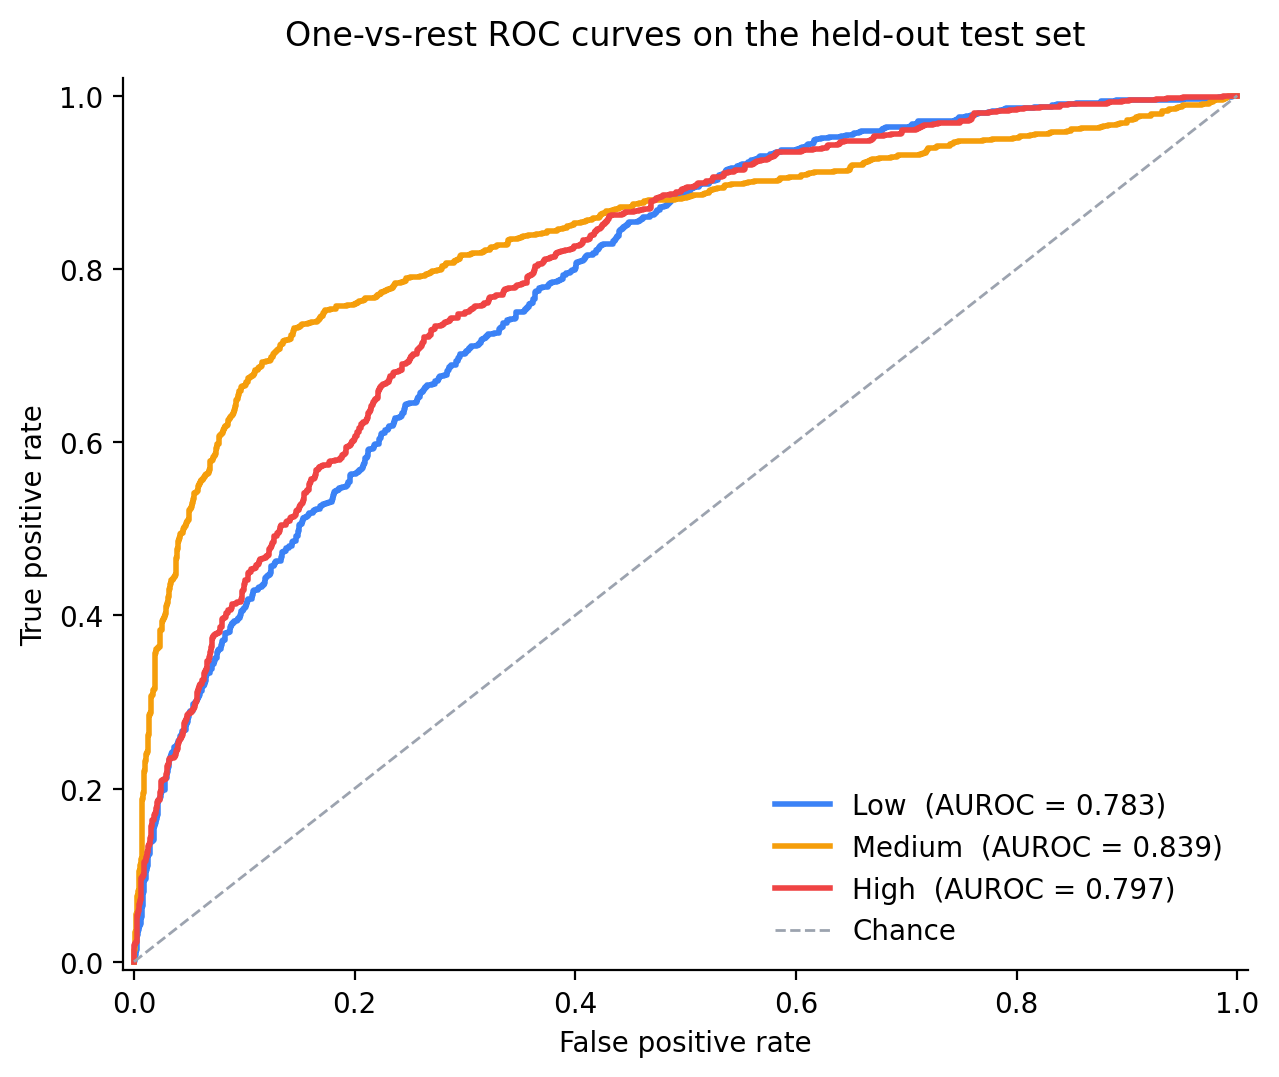
\includegraphics[width=0.70\textwidth]{figures/roc_curves.png}
\caption{One-vs-rest ROC curves on the test set. The macro-averaged AUROC is 0.806. The Medium class is typically the hardest in an ordinal binned task: it has neighbours on both sides, and the margin for error in either direction is smaller than for the two extreme classes.}
\label{fig:roc}
\end{figure}

\subsection{Interpretability: What is the Model Looking At?}

\begin{figure}[H]
\centering
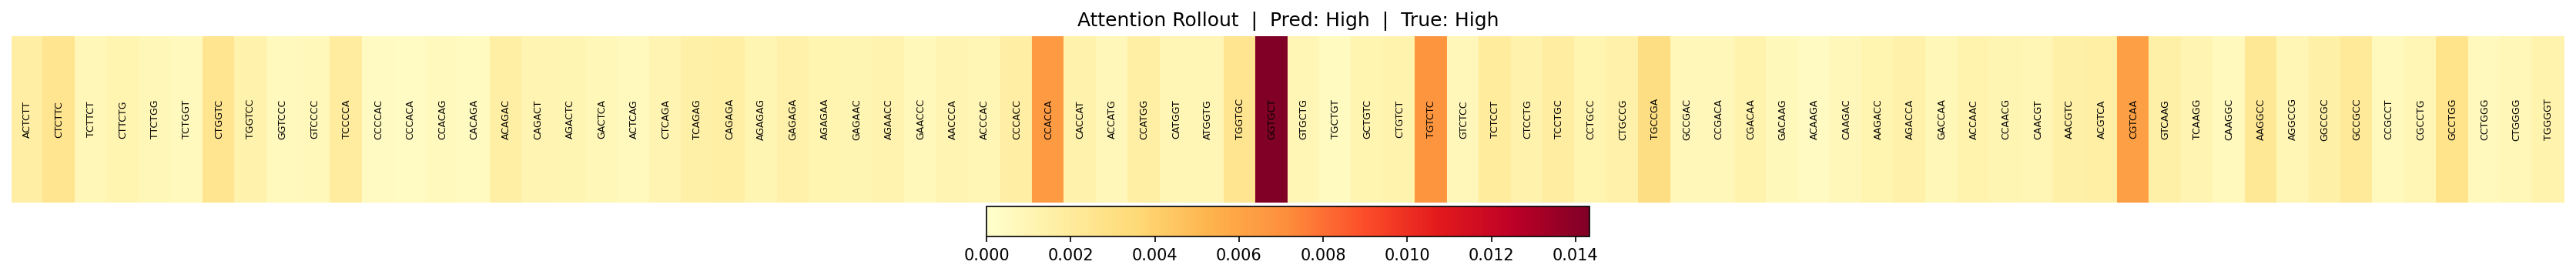
\includegraphics[width=0.95\textwidth]{figures/attention_hba1.png}
\caption{Attention rollout for \emph{HBA1} (haemoglobin alpha-1, classified High). Positions of high attention concentrate on a small number of regions in the sequence rather than spreading uniformly.}
\label{fig:attn_hba1}
\end{figure}

\begin{figure}[H]
\centering
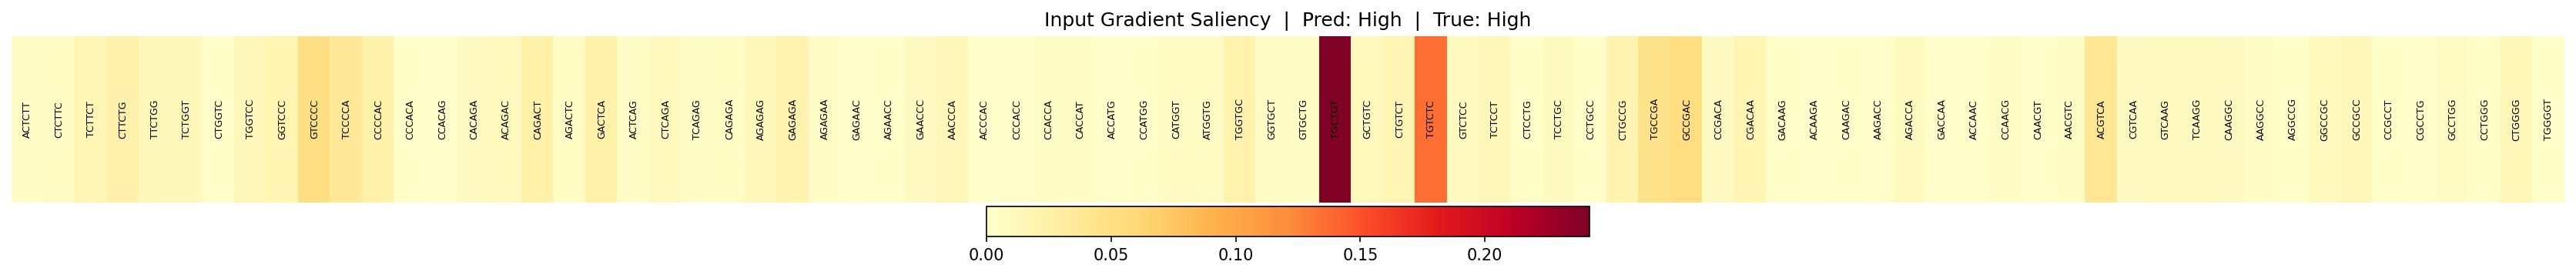
\includegraphics[width=0.95\textwidth]{figures/saliency_hba1.png}
\caption{Input-gradient saliency for the same gene. Saliency peaks broadly align with the attention rollout but distribute their mass more evenly along the sequence, suggesting that part of the signal is carried through the feed-forward sublayers rather than the attention mechanism.}
\label{fig:sal_hba1}
\end{figure}

The qualitative pattern across the three preloaded example genes (\emph{HBA1}, \emph{CCDC182}, \emph{IFNB1}) is consistent. When the model is confident, the two methods agree on a small number of clearly identifiable regions; when the model is uncertain, both maps go flat. That correspondence is not a proof of faithful explanation, but it makes the heatmaps a workable rough proxy for prediction confidence in practice. A biologist inspecting a borderline call can at least see which parts of the sequence the model is leaning on.

\subsection{The Web Application}

\begin{figure}[H]
\centering
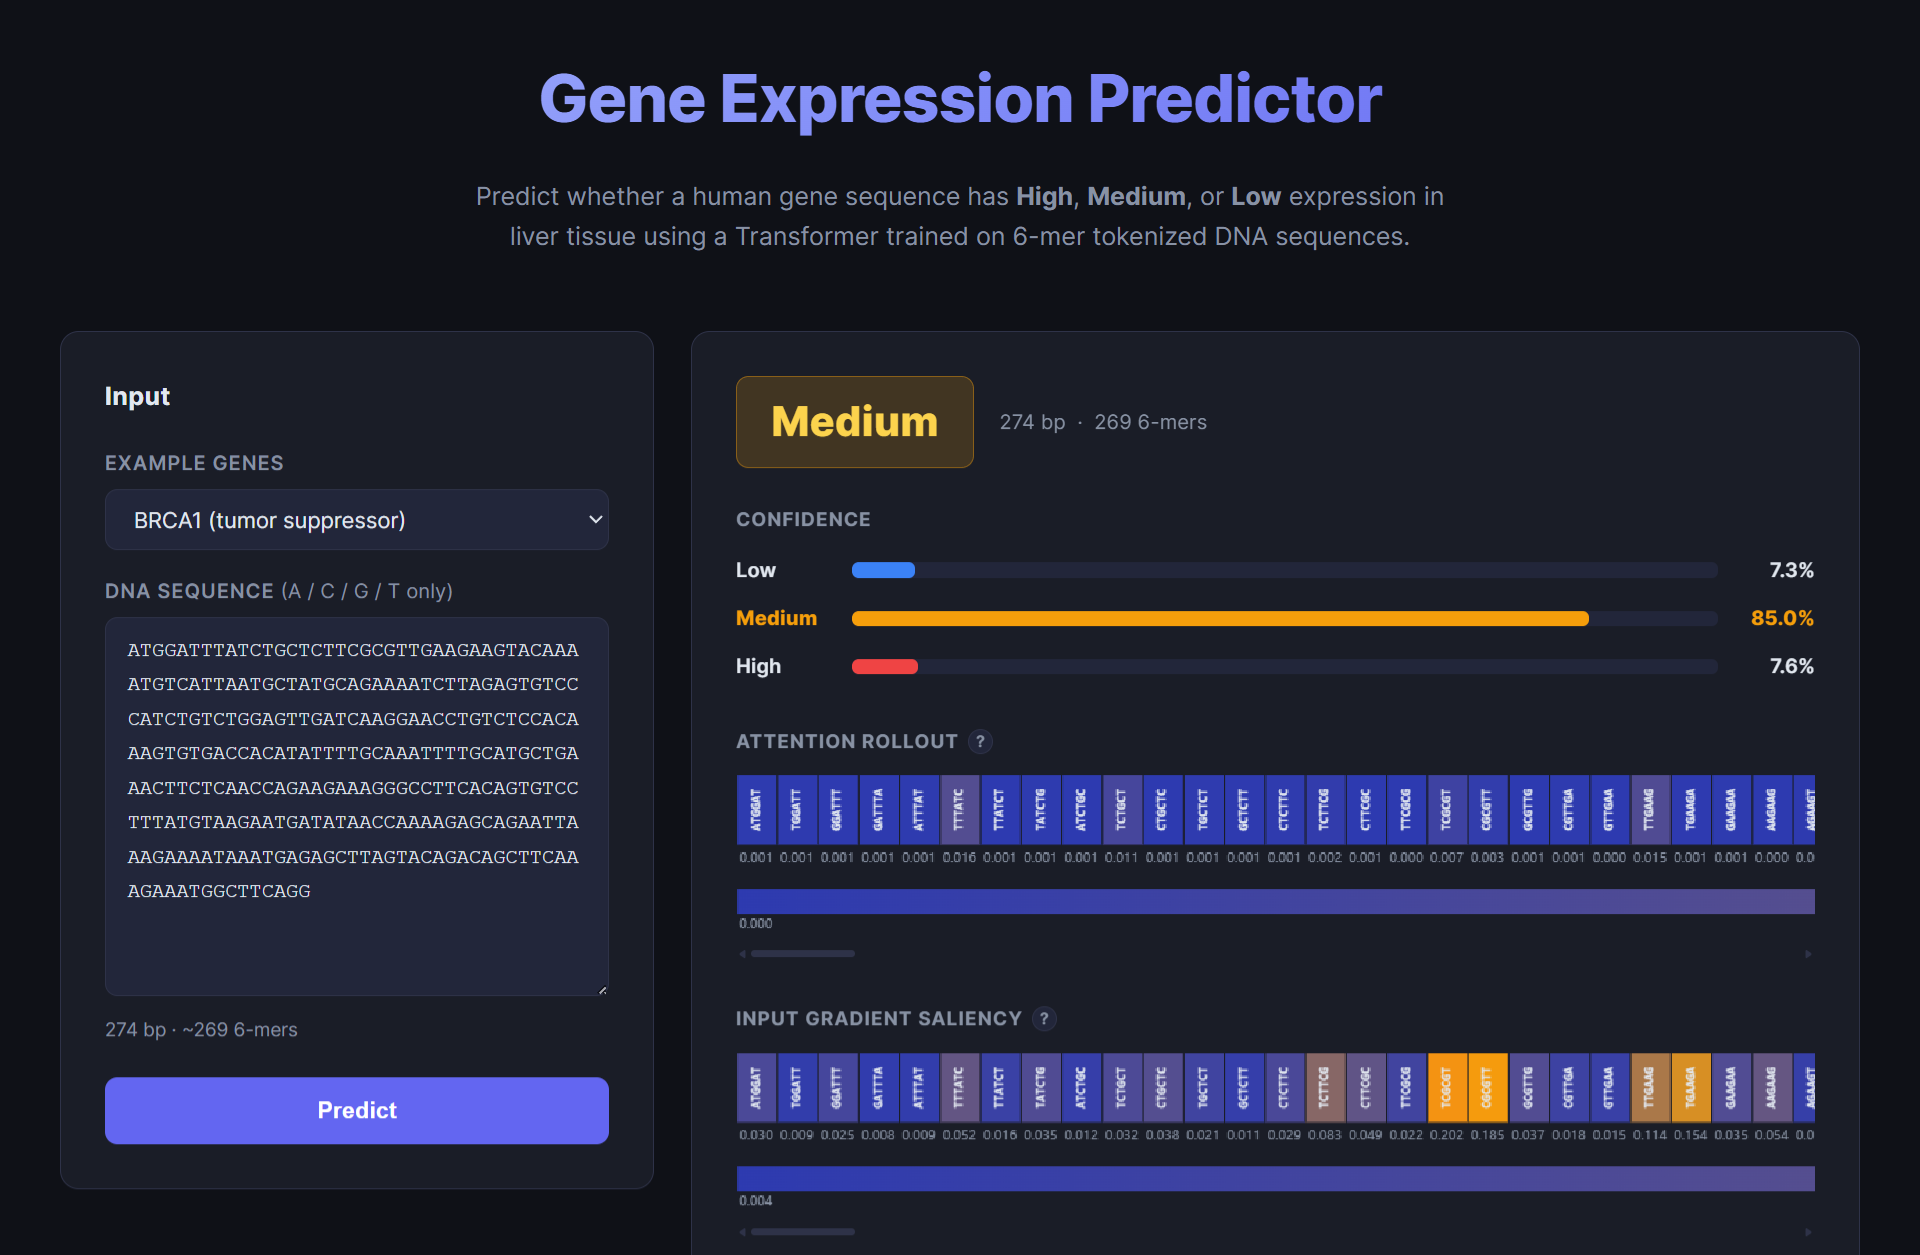
\includegraphics[width=0.85\textwidth]{figures/webapp_screenshot.png}
\caption{The FastAPI web interface. A user pastes a DNA sequence (or chooses a preloaded example: \emph{IFNB1} Low, \emph{CCDC182} Medium, \emph{HBA1} High), submits, and receives the predicted class, the full class-probability vector, the attention-rollout heatmap, and the saliency heatmap inline.}
\label{fig:webapp}
\end{figure}

The application is not the scientific contribution of the project, but it shapes how the project will be received. Reviewers and demo audiences engage with an interactive prediction in a way they do not engage with a static confusion matrix. The three preloaded example genes are chosen so the demo can walk through a confident-High prediction, a confident-Low prediction, and a borderline-Medium prediction in under a minute.

% ====================================================================
\section{Critical Evaluation and Limitations}

\subsection{Data Limitations}

The most consequential limitation is structural: the input is coding sequence only. Promoter regions, untranslated regions, distal enhancers, chromatin accessibility, and three-dimensional contact data are all absent. The known biology says these are where most of the expression-predictive signal lives, and excluding them caps how well any model on this input can do. The 63.4\% accuracy is best read as a measurement of how much expression-predictive signal sits inside the coding sequence specifically. That quantity is meaningful but limited, and the result reflects it.

The 1{,}000 base-pair length cap is a second constraint. It was chosen for computational reasons (positional encoding range and quadratic attention cost) but it biases the dataset toward shorter genes. Genes with long coding regions, many transcription factors and certain enzymes among them, are systematically underrepresented.

GTEx provides median TPM per tissue. We used liver. A gene that is silent in liver but active in brain (a neuron-specific synaptic protein, for instance) is labelled Low here, even though that label is not really a property of the gene's sequence in any tissue-agnostic sense. The labelling is internally consistent across the project but limits how the trained model generalises to other tissues.

\subsection{Design Limitations}

Three-class percentile binning is convenient but discards information. The codebase includes a regression head against $\log(\text{TPM})$ (\texttt{train.py --task regression}) that is not the primary reported result. Future work could compare classification and regression heads on the same data and report Spearman correlation or a similar rank-based metric, which would not be distorted by arbitrary class boundaries.

Reverse-complement augmentation assumes a kind of strand symmetry. For coding sequences this is a reasonable prior but not a perfect one. Codon structure is asymmetric, the direction of transcription matters, and treating a sequence and its reverse complement as fully interchangeable during training is a simplification.

Attention rollout is a useful but partial explanation method. It captures information flow within the attention mechanism only, and it cannot see the feed-forward sublayers, which carry a substantial fraction of a Transformer's computation. The saliency map covers some of that blind spot but is itself a noisy signal. Readers should treat the heatmaps as guides to model behaviour, not as causal accounts of why a given prediction was made.

The 6-mer vocabulary has a soft data-sparsity problem at the tail. The rarest 6-mers in our training set appear only a handful of times, and their embeddings are correspondingly under-trained. A byte-pair-encoding tokeniser would adapt the vocabulary to the data, at the cost of comparability with the standard k-mer convention used in DNA modelling.

% ====================================================================
\section{Conclusion}

We set out to find how well a Transformer could classify gene expression level from coding sequence alone, with no access to the regulatory regions biology says drive most of the variance. The answer is: meaningfully above chance, but well short of solved. The model reaches 63.4\% accuracy and a macro-F1 of 0.634 on a three-class balanced task. That is not a finished problem, but it is not noise either.

The result that probably matters most is the structure of the confusion matrix rather than the top-line accuracy. Errors stay close to the diagonal, and the model rarely confuses Low with High. An ordinal pattern emerging from a nominal loss function suggests the model is picking up real if limited information about expression level from features like codon usage, GC content, and local sequence composition. Pairing predictions with attention rollout and saliency turns the system from a black-box classifier into something a biologist can inspect at the level of individual 6-mers, and packaging the whole thing behind a FastAPI service makes the inspection interactive.

What we would not recommend doing with this model is treating it as a quantitative predictor of gene expression in any tissue. What it can do reasonably well is place a sequence into roughly the right region of the expression distribution, surface which parts of the sequence drove that placement, and serve as a starting point for the more interesting work of bringing regulatory context into the input.

% ====================================================================
\section{References}

\begin{enumerate}[label={[\arabic*]},leftmargin=*,itemsep=2pt]
    \item Vaswani, A., Shazeer, N., Parmar, N., Uszkoreit, J., Jones, L., Gomez, A.~N., Kaiser, {\L}., \& Polosukhin, I. (2017). Attention is all you need. \emph{Advances in Neural Information Processing Systems}, 30.
    \item Abnar, S., \& Zuidema, W. (2020). Quantifying attention flow in Transformers. \emph{Proceedings of the 58th Annual Meeting of the Association for Computational Linguistics}, 4190--4197.
    \item Simonyan, K., Vedaldi, A., \& Zisserman, A. (2014). Deep inside convolutional networks: visualising image classification models and saliency maps. \emph{Workshop at the International Conference on Learning Representations}.
    \item Loshchilov, I., \& Hutter, F. (2019). Decoupled weight decay regularization. \emph{International Conference on Learning Representations}.
    \item Szegedy, C., Vanhoucke, V., Ioffe, S., Shlens, J., \& Wojna, Z. (2016). Rethinking the Inception architecture for computer vision. \emph{Proceedings of the IEEE Conference on Computer Vision and Pattern Recognition}, 2818--2826.
    \item Xiong, R., Yang, Y., He, D., Zheng, K., Zheng, S., Xing, C., Zhang, H., Lan, Y., Wang, L., \& Liu, T.-Y. (2020). On layer normalization in the Transformer architecture. \emph{Proceedings of the 37th International Conference on Machine Learning}.
    \item GTEx Consortium. (2020). The GTEx Consortium atlas of genetic regulatory effects across human tissues. \emph{Science}, 369(6509), 1318--1330.
    \item Sayers, E.~W., Bolton, E.~E., Brister, J.~R., Canese, K., Chan, J., Comeau, D.~C., \emph{et al.} (2022). Database resources of the National Center for Biotechnology Information. \emph{Nucleic Acids Research}, 50(D1), D20--D26.
    \item Wu, C., MacLeod, I., \& Su, A.~I. (2013). BioGPS and MyGene.info: organizing online, gene-centric information. \emph{Nucleic Acids Research}, 41(D1), D561--D565.
\end{enumerate}

% ====================================================================
\section*{Appendix}

\subsection*{A. Expression Label Construction}

The rank-based percentile-binning step that converts continuous log-TPM into the three ordinal classes. Labels are assigned across the full dataset before the stratified train/val/test split, with rank ordering used in place of raw quantile thresholds to avoid bin-edge degeneracies when many genes share TPM = 0.

\begin{lstlisting}
import numpy as np
import pandas as pd

# compress the right tail of TPM
df['log_tpm'] = np.log(df['median_tpm'] + 1.0)

# rank-based binning handles ties (many TPM = 0 values) cleanly
n     = len(df)
ranks = df['log_tpm'].rank(method='first', ascending=True)

df['expression_label'] = 'Medium'
df.loc[ranks <= n * 0.33, 'expression_label'] = 'Low'
df.loc[ranks >  n * 0.67, 'expression_label'] = 'High'
\end{lstlisting}

\subsection*{B. Sample Inference Call}

A minimal client-side call against the FastAPI \texttt{/predict} endpoint:

\begin{lstlisting}
import requests

resp = requests.post(
    'http://127.0.0.1:8000/predict',
    json={'sequence': 'ATGGTGCTGTCTCCTGCCGACAAGACCAAC...'},
)
result = resp.json()

print(result['prediction'])      # 'High'
print(result['probabilities'])   # {'Low': 0.04, 'Medium': 0.15, 'High': 0.81}
\end{lstlisting}

\end{document}
